\subsection{Sleep/power­ down mode}\label{sleep}
Algorithms in this category try to minimise the time a node is active, and
maximise the time a node is asleep. A common approach to do this is to select
one or more masters from a set of nodes which take over the routing functionality
while the others can sleep safely. In such a scheme, nodes periodically wake up
and elect a new master if the current one goes away.

Two of the protocols discussed in this section, SPAN and GAF employ a master
slave approach, whereas the PEN protocol has no such concept.

\subsubsection{SPAN}\label{span}
%SPAN-FIGURE
In SPAN\cite{chen2002span}, a master is selected based on the following rule:
A node becomes a master if two of its neighbors cannot reach each other directly
or via one or two masters. For example, in Figure~\ref{spanmaster}, nodes B and
D become masters.

In order to prevent or at least reduce overloading of masters, masters periodically
check whether they should withdraw from being master; and non-master nodes
periodically check if they should become master.


\subsubsection{Geographic adaptive fidelity (GAF)}
\label{gaf}
\begin{figure*}[!t]
\subfloat[Grid example]{%
  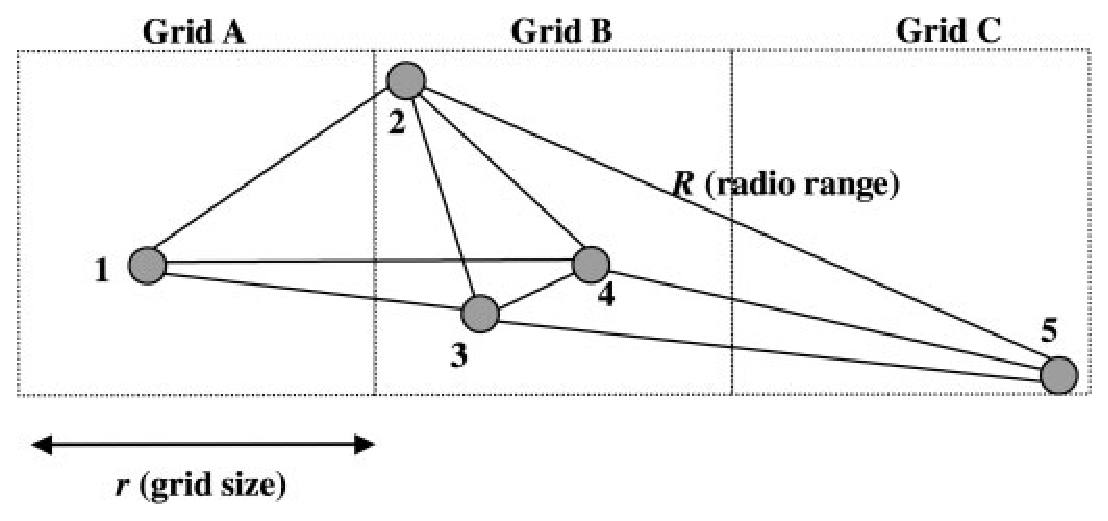
\includegraphics[width=0.46\textwidth]{images/gaf-grids}
  \label{gafgrids}
}
\hfill
\subfloat[Node states]{%
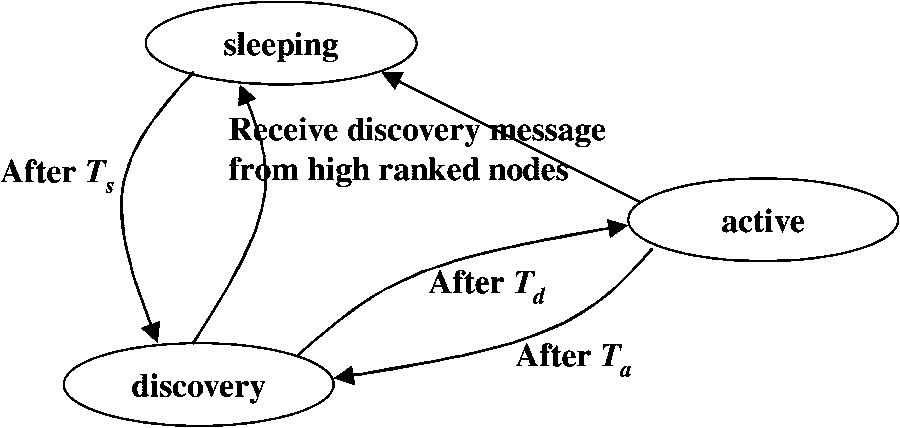
\includegraphics[width=0.46\textwidth]{images/gaf-states}
\label{gafstates}
}
\caption{Example grid and state diagram for GAF\cite{alotaibi2012survey}}
\end{figure*}
GAF\cite{xu2001geography} uses the geographical (GPS) location of a node in
order to position them into a virtual grid.

Within each grid, the node with the highest residual energy becomes the master
of the grid, responsible for routing messages through that grid, while the
slave nodes can be put to sleep and will alternate between sleep and listening
states. For example, in grid B of Figure~\ref{gafgrids}, one of 2,3,4 can be the
master of grid B and forward messages between A and B, while the other two can
be put to sleep.

Nodes have three states, as shown in Figure~\ref{gafstates}: active for some time span $T_{a}$, in which they
act as the master of the grid; discovery for some time span $T_{d}$, in which a
master is elected - a node becomes the master if it hears no more discover messages
for time span $T_{d}$; and finally, a node can be sleeping.


\subsubsection{Prototype embedded network (PEN)}\label{pen}
PEN\cite{girling2000design} does not follow the usual master-slave scheme
used by the other protocols. Nodes periodically wake up, advertise their
presence
by broadcast messages, and then listen for any communication requests before
powering down again.

A sending node waits until it receives a broadcast message from the intended
destination, then sends a communication request to the destination during
the destinations listening period. Finally, it starts the communication.

This scheme easily avoids the cost of selecting a master and avoids overloading
master nodes. It is only effective for networks without much traffic, as the delay
can be quite high because senders need to wait for receivers to wake up.
